\documentclass[11pt]{article}

\usepackage{booktabs}
\usepackage{dcolumn} 
\usepackage{epstopdf}
\usepackage{fourier}
\usepackage{fullpage}
\usepackage{graphicx}
\usepackage{hyperref}
\usepackage{longtable} 
\usepackage{natbib}
\usepackage{rotating}
\usepackage{tabularx}
\usepackage{amsmath}
\usepackage{algorithmic} 
\usepackage{algorithm2e}

\hypersetup{
  colorlinks = TRUE,
  citecolor=blue,
  linkcolor=red,
  urlcolor=black
}

\begin{document} 

\title{ kwow }

\date{\today}

\author{ John J. Horton \\ NYU Stern \footnote{ Author contact information, datasets and code are currently or will be available at \href{http://www.john-joseph-horton.com/}{http://www.john-joseph-horton.com/}. } }
\maketitle

\begin{abstract}
\noindent  Here is a really great abstract.  \newline
\noindent JEL J01, J24, J3
\end{abstract} 

\section{Introduction}
\cite{smith1999wealth} had some great ideas! 

\subsection{Plots!}

\begin{figure}[h]
  \begin{center}
  \caption{Here is a figure} \label{fig:hist}
  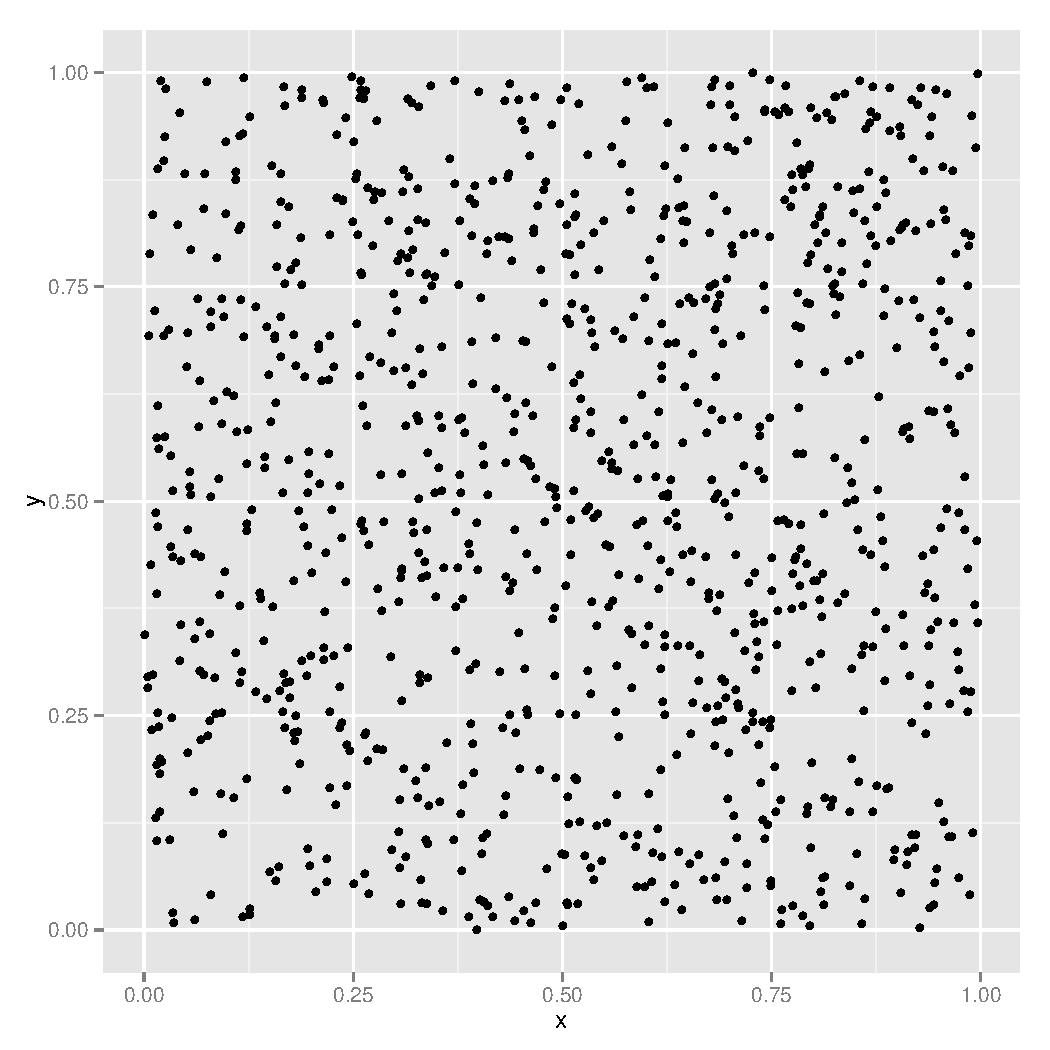
\includegraphics[scale=0.25]{./plots/hist.pdf}
  \end{center} 
\end{figure}

\bibliographystyle{aer}
\bibliography{kwow.bib}

\end{document} 
